\newpage
\chapter*{\centering{\MakeUppercase{PHẦN I: TƯ DUY MÁY TÍNH}}}
\addcontentsline{toc}{chapter}{\textcolor{fitblue}{\MakeUppercase{PHẦN I: TƯ DUY MÁY TÍNH}}}

\noindent \indent Phần đầu của cuốn sách này giới thiệu về tư duy máy tính như một cách tiếp cận để giải quyết vấn đề. Nó giới thiệu các khái niệm cơ bản và giúp độc giả xây dựng sự hiểu biết vững chắc về chúng. Bên cạnh các khái niệm lý thuyết, bạn sẽ tìm thấy các định nghĩa, mẹo, cảnh báo, quy tắc vàng và các cơ hội để đọc thêm ở những nguồn tài liệu khác.

Phần này không yêu cầu bất kỳ kỹ năng lập trình nào từ phía độc giả. Các ví dụ minh họa được xây dựng dựa trên những khái niệm thường ngày đến từ nhiều lĩnh vực khác nhau. Ở cuối mỗi chương, bạn sẽ có cơ hội kiểm tra kiến thức mới tiếp thu của mình bằng cách thực hiện một số bài tập. Giống như các ví dụ, những bài tập này không đòi hỏi kỹ năng lập trình trước đó.

Sau khi đọc phần này, bạn sẽ có được sự hiểu biết về tất cả các chủ đề cấu thành nên tư duy máy tính. Khi đó, bạn sẽ sẵn sàng cho Phần II, nơi bạn sẽ học cách vận dụng những kỹ năng đó vào thực tế với tư cách là một lập trình viên. 

% =================SEC================
\section*{1. Tư duy máy tính là gì?}
\addcontentsline{toc}{section}{\textcolor{black}{1. Tư duy máy tính là gì?}}

\subsection*{1.1. Mục tiêu}
\addcontentsline{toc}{subsection}{\textcolor{black}{1.1. Mục tiêu}}
\begin{itemize}
    \item Định nghĩa tư duy máy tính.
    \item Chỉ ra cách nó có thể được sử dụng trong các lĩnh vực khác nhau.
    \item Giải thích các hạn chế hiện tại của tư duy máy tính.
\end{itemize}

\subsection*{1.2. Tư duy máy tính là gì?}
\addcontentsline{toc}{subsection}{\textcolor{black}{1.2. Tư duy máy tính là gì?}}

\begin{itemize}
    \item Trả lời câu hỏi này thực sự là một thách thức lớn. Những người ủng hộ tư duy máy tính (\texttt{CT}), cho đến tận gần đây, đã dành rất nhiều thời gian để tranh luận về cách định nghĩa nó.

    \item Gần đây nhất là vào năm 2011, một hội thảo đã được tổ chức để nhiều cá nhân cùng nhau khám phá bản chất của \texttt{CT} nên là gì. Một số người tại hội thảo này đã lập luận ủng hộ một định nghĩa chặt chẽ và nhất quán (\texttt{Committee for the Workshops on Computational Thinking, 2011}). Ngược lại, những người khác lại cho rằng việc cố gắng định nghĩa \texttt{CT} một cách nghiêm ngặt là không cần thiết (\texttt{Voogt et al., 2015}).

    \item Theo quan điểm của nhóm sau, việc hiểu về \texttt{CT} không nên được thực hiện bằng cách đưa ra một định nghĩa theo nghĩa thông thường (nói cách khác, tạo ra một danh sách các điều kiện mà một thứ gì đó phải đáp ứng trước khi được coi là phù hợp). Voogt và các cộng sự lập luận rằng việc định nghĩa \texttt{CT} cũng gặp phải những khó khăn tương tự như việc định nghĩa một \texttt{``trò chơi''} là gì. (Có phải mọi trò chơi đều phải có ít nhất một người chơi đấu với người khác? Có phải mọi trò chơi đều có khái niệm chiến thắng? Có phải mọi trò chơi đều nên bao gồm một số yếu tố may rủi hoặc ngẫu nhiên?) Giống như cách chúng ta hiểu về một trò chơi, họ nói rằng, cách tiếp cận để định nghĩa \texttt{CT} nên \verb|mờ| (\verb|fuzzier|) hơn và được xem như một chuỗi các điểm tương đồng và mối quan hệ đan xen, chồng lấp lên nhau.

    \item Còn những lý do khác khiến việc định nghĩa \texttt{CT} trở thành một nỗ lực đầy thách thức. Thứ nhất, tư duy máy tính có liên quan chặt chẽ với \texttt{CS}, lĩnh vực mà bản thân nó cũng có thể gặp khó khăn để định nghĩa một cách thỏa đáng. Giống như \texttt{CS}, \texttt{CT} bao gồm một loạt các ý tưởng cả trừu tượng và cụ thể. Cả hai đều có chung tính ứng dụng phổ quát, và sự rộng lớn này, mặc dù tạo nên sức mạnh, nhưng cũng khiến \texttt{CT} khó có thể được định nghĩa một cách súc tích.

    \item \texttt{CT} cũng là một ý tưởng vừa mới vừa cũ. Nó mới theo nghĩa là chủ đề này đột ngột trở thành một đề tài tranh luận sôi nổi vào năm 2006 sau bài phát biểu của \texttt{Wing (2006)}. Tuy nhiên, nhiều ý tưởng cốt lõi của nó đã được thảo luận trong vài thập kỷ, và trong quá trình đó, mọi người đã đóng gói chúng theo những cách khác nhau.

    \item Ví dụ, ngay từ năm 1980, \texttt{Seymour Papert} từ \texttt{Viện Công nghệ Massachusetts} đã tiên phong trong một kỹ thuật mà ông gọi là \verb|``tư duy thủ tục''| (\verb|procedural thinking|) (\texttt{Papert, 1980}). Nó chia sẻ nhiều ý tưởng với những gì chúng ta nghĩ về \texttt{CT} hiện nay. Thông qua tư duy thủ tục, Papert nhằm mục đích cung cấp cho sinh viên một phương pháp giải quyết vấn đề bằng cách sử dụng máy tính làm công cụ. Ý tưởng là sinh viên sẽ học cách tạo ra các giải pháp thuật toán mà sau đó máy tính có thể thực hiện; để làm điều này, ông đã sử dụng ngôn ngữ lập trình \texttt{Logo}. Các bài viết của Papert đã truyền cảm hứng cho nhiều nội dung trong \texttt{CT}, mặc dù \texttt{CT} đã đi chệch khỏi ý tưởng ban đầu này ở một số khía cạnh.

    \item Tuy nhiên, trong suốt 10 năm sau bài phát biểu của \texttt{Wing}, một số định nghĩa súc tích đã được thử nghiệm. Một mẫu nhỏ trong số đó được trình bày trong Bảng 1.1. Mặc dù chúng gợi ý về những ý tưởng tương đồng, nhưng dường như có sự đa dạng trong những gì các tác giả này phát biểu. Có lẽ \texttt{Voogt} và các cộng sự đã đúng, và hy vọng tốt nhất của chúng ta để hiểu về \texttt{CT} là xây dựng dựa trên những khái niệm chồng lấp, đan xen đó.

    \item Thật may mắn, công việc này đã được thực hiện bởi \texttt{Cynthia Selby} (\texttt{Selby, 2013}), khi bà rà soát các tài liệu về \texttt{CT} để tìm kiếm các khái niệm và chia chúng thành hai loại: các khái niệm cốt lõi của \texttt{CT}, và các khái niệm mang tính ngoại vi (\verb|peripheral|) nên được loại trừ khỏi một định nghĩa.
\end{itemize}

\begin{table}[H]
\centering
\renewcommand{\arraystretch}{1.4}
\begin{tabular}{|p{10cm}|p{4cm}|}
\hline
\textbf{Định nghĩa} & \textbf{Nguồn} \\ \hline

``Tư duy máy tính là các quy trình tư duy liên quan đến việc hình thành một vấn đề và biểu diễn (các) giải pháp của nó theo cách mà một máy tính—con người hoặc máy móc—có thể thực hiện một cách hiệu quả.'' 
& (Wing, 2014) \\ \hline

``Hoạt động trí tuệ nhằm trừu tượng hóa các vấn đề và hình thành các giải pháp có thể được tự động hóa.'' 
& (Yadav và cộng sự, 2014) \\ \hline

``Quy trình nhận diện các khía cạnh của tính toán trong thế giới xung quanh chúng ta, và áp dụng các công cụ cũng như kỹ thuật từ Khoa học máy tính để hiểu và lập luận về cả các hệ thống và quy trình tự nhiên lẫn nhân tạo.'' 
& (Furber, 2012) \\ \hline

``Một sự định hướng trí tuệ để hình thành các vấn đề dưới dạng sự chuyển đổi từ một số đầu vào thành đầu ra và tìm kiếm các thuật toán để thực hiện các chuyển đổi đó. Ngày nay, thuật ngữ này đã được mở rộng để bao gồm việc tư duy với nhiều cấp độ trừu tượng, sử dụng toán học để phát triển các thuật toán, và xem xét mức độ mở rộng (khả năng co giãn) của một giải pháp trên các quy mô vấn đề khác nhau.'' 
& (Denning, 2009) \\ \hline

``[Dạy CT là dạy] cách tư duy như một nhà kinh tế học, một nhà vật lý học, một nghệ sĩ, và để hiểu cách sử dụng tính toán nhằm giải quyết các vấn đề của họ, để sáng tạo và để khám phá những câu hỏi mới có thể được nghiên cứu một cách hiệu quả.'' 
& (Hemmendinger, 2010) \\ \hline

\end{tabular}
\caption*{Bảng 1.1: Danh sách các định nghĩa về tư duy máy tính}
\end{table}

\begin{itemize}
    \item Trong cuốn sách này, tôi sẽ tuân theo một cách tiếp cận rất giống với \texttt{Selby}. Một số khái niệm nhất định được coi là \verb|"cốt lõi"| đối với \texttt{CT} và được trình bày rất chi tiết. Những khái niệm khác cũng được đưa vào, nhưng được xem là ngoại vi và được trình bày ít chi tiết hơn nhiều.

    \item Cuốn sách này xem xét các khái niệm cốt lõi của \texttt{CT} bao gồm:
    \begin{itemize}
        \item Tư duy logic (\texttt{logical thinking});
        \item Tư duy thuật toán (\texttt{algorithmic thinking});
        \item Sự phân rã (\texttt{decomposition});
        \item Tổng quát hóa và nhận dạng mẫu (\texttt{generalisation and pattern recognition});
        \item Mô hình hóa (\texttt{modelling});
        \item Sự trừu tượng hóa (\texttt{abstraction});
        \item Sự đánh giá (\texttt{evaluation}).
    \end{itemize}

    \item Các khái niệm ngoại vi khác sẽ được đề cập, nhưng không được xem là thiết yếu đối với chủ đề \texttt{CT}. Chúng bao gồm:
    \begin{itemize}
        \item Biểu diễn dữ liệu (\texttt{data representation});
        \item Tư duy phản biện (\texttt{critical thinking});
        \item Khoa học máy tính (\texttt{computer science});
        \item Tự động hóa (\texttt{automation});
        \item Mô phỏng/Trực quan hóa (\texttt{simulation/visualisation}).
    \end{itemize}

    \item Tôi sẽ định nghĩa từng khái niệm cụ thể khi chúng được giới thiệu trong suốt nội dung của cuốn sách.
\end{itemize}

\subsection*{1.3. Tư duy máy tính được sử dụng như thế nào?}
\addcontentsline{toc}{subsection}{\textcolor{black}{1.3. Tư duy máy tính được sử dụng như thế nào?}}
\begin{itemize}
    \item \texttt{CT} có thể được áp dụng bởi bất kỳ ai đang cố gắng giải quyết một vấn đề mà trong đó máy tính đóng một vai trò trong giải pháp. Để giúp chúng ta có một số ý niệm về cách \texttt{CT} được sử dụng — không chỉ trong khoa học máy tính mà còn trong một loạt các lĩnh vực khác nhau — chúng ta có thể xem xét các ví dụ (nguồn từ \texttt{Barr và Stephenson (2011)}) về các khái niệm cốt lõi của tư duy máy tính vừa được liệt kê.

    \item Ví dụ, tư duy thuật toán có thể có ý nghĩa gì trong các tình huống khác nhau? Đối với một nhà khoa học máy tính, đó là việc nghiên cứu các thuật toán và ứng dụng của chúng vào các vấn đề khác nhau. Đối với một nhà toán học, nó có thể là việc thực hiện phép chia dài (\verb|long division|), phân tích nhân tử hoặc thực hiện các phép nhớ trong phép cộng hoặc phép trừ. Một nhà khoa học có thể coi đó là quy trình thực hiện một trình tự thực nghiệm.

    \item Tương tự, sự trừu tượng hóa có ứng dụng vượt ra ngoài góc nhìn của nhà khoa học máy tính. Khi một nhà ngôn ngữ học sử dụng phép so sánh và ẩn dụ, hoặc viết một câu chuyện có các nhánh rẽ, họ đang sử dụng sự trừu tượng hóa; các nhà khoa học xã hội cũng vậy khi họ tóm tắt các sự thật và sử dụng chúng để đưa ra kết luận. Khi một nhà khoa học xây dựng một mô hình hoặc một nhà toán học sử dụng đại số, họ cũng đã đưa sự trừu tượng hóa vào công việc của mình.

    \item Dưới đây là các ví dụ từ những nguồn khác thảo luận về các trường hợp cụ thể của \texttt{CT} trong thực tế.

    \item \textbf{Ví dụ: Thiết lập đường ống (Pipelining) cho một lễ tốt nghiệp}
    \begin{itemize}
        \item Trưởng khoa Randy Bryant đã cân nhắc cách làm cho lễ trao bằng tại buổi lễ tốt nghiệp diễn ra nhanh hơn. Bằng cách sắp xếp cẩn thận vị trí đứng của từng cá nhân, ông đã thiết kế một đường ống (\verb|pipeline|) hiệu quả để khi Trợ lý Trưởng khoa Mark Stehlik đọc tên và danh hiệu của mỗi sinh viên tốt nghiệp, người đó có thể nhận bằng, sau đó nhận một cái bắt tay hoặc cái ôm từ Mark, và sau đó được chụp ảnh. Đường ống này cho phép một dòng sinh viên di chuyển liên tục qua sân khấu (mặc dù một sự tắc nghẽn đường ống — \verb|pipeline stall| — đã xảy ra bất cứ khi nào mũ tốt nghiệp của sinh viên bị đổ khi đang nhận cái ôm từ Mark). (\texttt{Wing, 2011})
    \end{itemize}

    \item \textbf{Ví dụ: Dự báo biến đổi khí hậu}
    \begin{itemize}
        \item Dự báo biến đổi khí hậu toàn cầu chỉ có thể thực hiện được nhờ vào các mô hình máy tính tiên tiến. Theo \texttt{Cơ quan Khí tượng Vương quốc Anh (UK Met Office)}: "Cách duy nhất để dự báo thời tiết hàng ngày và những thay đổi của khí hậu trong khoảng thời gian dài hơn là sử dụng các mô hình máy tính." (\texttt{Furber, 2012})
    \end{itemize}

    \item \textbf{Ví dụ: Sắp xếp các bản phổ nhạc}
    \begin{itemize}
        \item "Tôi đến một buổi biểu diễn của ban nhạc lớn (big band), và người trưởng nhóm đưa ra các cuốn sách với khoảng 200 bản phổ nhạc chưa được sắp xếp cùng một danh sách bài diễn gồm khoảng 40 tiêu đề mà chúng tôi phải lấy ra và sắp xếp theo thứ tự để sẵn sàng chơi. Mọi người khác bắt đầu tìm kiếm trong chồng tài liệu, rút từng bản phổ nhạc một. Tôi quyết định sắp xếp 200 bản phổ nhạc đó theo thứ tự bảng chữ cái $O(N \log N)$ rồi sau đó mới rút các bản nhạc ra $O(M \log(N))$. Tôi vẫn đang sắp xếp khi các thành viên khác đã tìm xong một nửa số bản nhạc của họ và tôi bắt đầu nhận được vài cái nhìn kỳ quặc, nhưng cuối cùng, tôi lại là người hoàn thành đầu tiên. Đó chính là tư duy máy tính." (\texttt{Roger Dannenberg trong Wing, 2011})
    \end{itemize}

    \item \textbf{Ví dụ: Hỗ trợ cảnh sát, luật sư và thẩm phán}
    \begin{itemize}
        \item Tư duy máy tính có một truyền thống lâu đời trong việc ảnh hưởng đến luật pháp, đặc biệt là trong giấc mơ cung cấp một bộ quy tắc logic có thể tự động hóa quy trình đưa ra phán quyết, \verb|[làm nền tảng]| cho mong muốn giảm thiểu sự tự ý của con người và tối đa hóa khả năng dự đoán của kết quả... các hệ thống lập luận pháp lý đã và đang tạo ra những bước tiến khi chúng cố gắng hỗ trợ những người đưa ra quyết định pháp lý. Ví dụ, các nghiên cứu tại Trung tâm Joseph Bell đã xây dựng một hệ thống thiết lập một không gian các giả thuyết để giải thích các bằng chứng tại hiện trường vụ án. Hệ thống này đã được sử dụng để nhắc nhở các thám tử về những giả thuyết mà lẽ ra họ có thể đã bỏ qua. (\texttt{Bundy, 2007})
    \end{itemize}

\end{itemize}

\subsection*{1.4. Các lưu ý làm rõ}
\addcontentsline{toc}{subsection}{\textcolor{black}{1.4. Các lưu ý làm rõ}}

\begin{itemize}
    \item Phần này thảo luận về những hiểu lầm phổ biến về \texttt{CT}, cũng như những thiếu sót hiện tại của nó.

    \item \textbf{Tư duy máy tính không phải là gì?}
    \begin{itemize}
        \item Chắc chắn sẽ có một số nhầm lẫn về việc \texttt{CT} là gì và không phải là gì. Một mặt, nó liên quan chặt chẽ đến các môn học khác như khoa học máy tính và lập trình, và việc phân biệt giữa chúng có thể gặp khó khăn. Mặt khác, định nghĩa của nó rất rộng và đã là chủ đề tranh luận trong nhiều năm. Phần này sẽ thảo luận về một số điều mà một số người có thể đã tin về \texttt{CT} nhưng không nhất thiết là đúng. Trong quá trình đó, nhiều chi tiết hơn về bản chất của \texttt{CT} sẽ được hé lộ.

        \item Thứ nhất, dạy tư duy máy tính không giống như dạy khoa học máy tính. Mục tiêu chính của việc dạy khoa học máy tính là giáo dục sinh viên về việc nghiên cứu và ứng dụng các nguyên lý tính toán toán học. Có lẽ để phản bác lại ấn tượng này, một số người, bao gồm cả \texttt{Jeannette Wing}, đã nói rằng tư duy máy tính là \verb|"tư duy như một nhà khoa học máy tính"|. Tuy nhiên, những người khác đã chỉ trích cụm từ này (ví dụ: \texttt{Denning, 2009; Hemmendinger, 2010}) vì nó để lại một sự liên tưởng mạnh mẽ với khoa học máy tính, điều này dẫn đến rủi ro là mọi người xem nó không phải như một kỹ năng hàng ngày, mà chỉ đơn thuần là một sự \verb|"đóng gói lại"| của \texttt{CS}.

        \item Dạy lập trình (một lĩnh vực con của \texttt{CS}) chủ yếu được thực hiện để giáo dục sinh viên cách tốt nhất để viết chương trình, và nó tập trung vào việc tạo ra phần mềm chất lượng cao. \texttt{CT}, mặc dù chia sẻ một số khía cạnh với các môn học này, nhưng được mô tả chính xác hơn như là một cách tiếp cận để giải quyết vấn đề. Điều làm cho nó khác biệt với các cách tiếp cận giải quyết vấn đề khác là \texttt{CT} giả định rằng một máy tính sẽ thực thi giải pháp cuối cùng.

        \item \texttt{CT} dạy một cách tiếp cận giải quyết vấn đề mà mục tiêu cuối cùng là cung cấp một giải pháp có hình thức sẵn sàng để được lập trình vào máy tính.

        \item \texttt{CT} lấy một tập hợp tương đối nhỏ các khái niệm – những khái niệm vốn dĩ quan trọng đối với \texttt{CS} – và sử dụng chúng để xây dựng một cách tiếp cận giải quyết vấn đề có khả năng ứng dụng rộng rãi.

        \item Những sự phân biệt này rất quan trọng. Việc dạy các kỹ năng tin học như một phần bắt buộc trong chương trình giảng dạy ở trường học đã được thử nghiệm ở nhiều nơi trên thế giới. Mặc dù những nỗ lực này là cao cả và đáng giá, nhưng bằng chứng vẫn chưa kết luận được liệu chúng có thành công hay không trong mục tiêu dạy các kỹ năng có thể chuyển đổi (\verb|transferable skills|) (\texttt{Voogt et al., 2015}); nghĩa là, những kỹ năng mà học sinh có thể mang theo vào các lĩnh vực khác nhau một cách trực quan. \texttt{CT} nỗ lực thực hiện tốt hơn ở khía cạnh này. Bằng cách chắt lọc một số khía cạnh cốt lõi của \texttt{CS} có liên quan đến nhiều lĩnh vực khác, \texttt{CT} có thể trở thành một khóa học trong chương trình giảng dạy cốt lõi ở trường học phù hợp với tất cả mọi người. Ví dụ, trong chương trình giảng dạy tin học của \texttt{Vương quốc Anh}, \texttt{CT} đã đóng một vai trò lớn (\texttt{Bộ Giáo dục, 2013}). Nó thậm chí có thể là một phần của khóa học \texttt{CS} hoặc lập trình tập trung riêng biệt vào việc giải quyết vấn đề dựa trên máy tính.

        \item Khi nhấn mạnh sự khác biệt giữa khoa học máy tính và tư duy máy tính, cũng cần chỉ ra rằng các khái niệm \texttt{CT} khó có thể là độc quyền của \texttt{CS}. Như \texttt{David Hemmendinger (2010)} chỉ ra: "Xây dựng mô hình, tìm và sửa lỗi, vẽ sơ đồ, phân tích – tất cả đều là các phần của hoạt động khoa học (và các hoạt động khác)." Ví dụ, các nhà khoa học tự nhiên từ lâu đã ủng hộ rằng tính toán là \verb|"chân thứ ba"| của quy trình khoa học (bên cạnh lý thuyết và thực nghiệm) và tư duy máy tính là thiết yếu đối với công việc của họ (\texttt{Denning, 2009}).

        \item Mục tiêu cuối cùng không phải là dạy mọi người tư duy như một nhà khoa học máy tính, mà là dạy họ áp dụng các yếu tố chung này để giải quyết vấn đề và khám phá những câu hỏi mới có thể được nghiên cứu trong và giữa tất cả các ngành học. (\texttt{Barr và Stephenson, 2011})
    \end{itemize}

    \item \textbf{Những thiếu sót hiện tại}
    \begin{itemize}
        \item Chúng ta sẽ sớm tiến hành xem xét chi tiết về tư duy máy tính. Tuy nhiên, trước khi điều đó diễn ra, một cuộc thảo luận trung thực về chủ đề này ở dạng thức hiện tại nên được trình bày thẳng thắn với bất kỳ thiếu sót nào. Hãy nhớ rằng những điều này có thể biến mất khi \texttt{CT} trở nên trưởng thành hơn.

        \item \textbf{Tính trưởng thành}
        \begin{itemize}
            \item Mặc dù nó có những ảnh hưởng và tiền thân từ cách đây vài thập kỷ, \texttt{CT} với tư cách là một khái niệm chính thức vẫn còn tương đối non trẻ. Các hội thảo để khám phá ý nghĩa của \texttt{CT} chỉ mới được tổ chức 5 năm trước khi cuốn sách này được viết. Chỉ cách đây 3 năm, \texttt{Cynthia Selby} đã viết một bài báo quan trọng đề xuất một định nghĩa cho \texttt{CT} (\texttt{Selby, 2013}), bởi vì các định nghĩa vào thời điểm đó vẫn còn mơ hồ. Hầu hết các ngành học khác đã ngừng tổ chức các cuộc họp mặt để quyết định chính xác họ làm gì từ lâu. Tuy nhiên, một sự đồng thuận hiện đang hình thành về những gì cần đưa vào một định nghĩa, phần lớn phù hợp với đề xuất của Selby về \texttt{CT} là: "một cách tiếp cận tập trung vào giải quyết vấn đề, kết hợp các quy trình tư duy sử dụng sự trừu tượng hóa, sự phân rã, các thuật toán, sự đánh giá và sự tổng quát hóa" (2013). 
        \end{itemize}

        \item \textbf{Hiệu quả}
        \begin{itemize}
            \item Một hệ quả khác của sự non trẻ của \texttt{CT} là sự khan hiếm tương đối các bằng chứng về việc giảng dạy \texttt{CT} thực sự hiệu quả như thế nào. Cho đến nay, nó vẫn chưa được giảng dạy rộng rãi trong một thời gian dài. Tuy nhiên, khối lượng bằng chứng sẽ tăng lên khi các nghiên cứu về tính hiệu quả của nó được tiến hành. Các báo cáo kinh nghiệm và chứng thực cung cấp một dạng bằng chứng tức thời hơn.
        \end{itemize}

        \item \textbf{Nhận thức về tính áp đặt}
        \begin{itemize}
            \item Các nhà bình luận khác đã cảnh báo rằng những người ủng hộ \texttt{CT} có nguy cơ trở nên mang tính \verb|"áp đặt"| (\verb|imperialistic|) và gây khó chịu. Những tuyên bố của họ như \verb|"bạn nên tư duy như một nhà khoa học máy tính"| hoặc "tư duy máy tính là X" (trong đó X là thứ mà họ chấp thuận) có vẻ mang tính xác lập lãnh địa. Như \texttt{David Hemmendinger (2010)} đã nói, những người ủng hộ nên cẩn thận để \texttt{CT} không rơi vào thói quen nói rằng: "Nếu đó là một cách tư duy tốt, thì đó là của chúng tôi." Cần lưu ý rằng nhiều thực hành trong \texttt{CT} không phải là nguyên bản của chủ đề này. Trên thực tế, không phải tất cả chúng đều là nguyên bản của khoa học máy tính; nhiều điều trong số đó đã được sử dụng trong các lĩnh vực khác cũng như cuộc sống hàng ngày từ lâu. chúng không đơn giản trở thành \verb|"thuộc về máy tính"| chỉ nhờ vào việc tìm thấy ứng dụng trong tính toán.
        \end{itemize}

        \item Tuy nhiên, sự non trẻ của \texttt{CT} phần nào được giảm bớt khi bạn nhận ra rằng các thành phần cấu thành của nó (chẳng hạn như logic, thuật toán và sự phân rã) đều đã được thử nghiệm, kiểm chứng và trưởng thành một cách riêng lẻ.
    \end{itemize}

\end{itemize}

\subsection*{1.5. Bài tập}
\addcontentsline{toc}{subsection}{\textcolor{black}{1.5. Bài tập}}

\begin{itemize}
    \item \textbf{BÀI TẬP 1}
    \begin{itemize}
        \item Liệt kê các khái niệm cốt lõi của \texttt{CT} (Tư duy máy tính).
    \end{itemize}

    \item \textbf{BÀI TẬP 2}
    \begin{itemize}
        \item Đưa ra một ví dụ về cách bạn nghĩ những người trong mỗi nghề nghiệp sau đây tư duy theo hướng máy tính:
        \begin{itemize}
            \item A. Nhà toán học;
            \item B. Nhà khoa học;
            \item C. Kỹ sư;
            \item D. Nhà ngôn ngữ học.
        \end{itemize}
    \end{itemize}

    \item \textbf{BÀI TẬP 3}
    \begin{itemize}
        \item Hãy nghĩ về các hoạt động hàng ngày mà bạn tham gia có liên quan đến tư duy máy tính.
    \end{itemize}
\end{itemize}

% =================SEC================
\section*{2. Tư duy logic và thuật toán}
\addcontentsline{toc}{section}{\textcolor{black}{2. Tư duy logic và thuật toán}}

\subsection*{2.1. Mục tiêu}
\addcontentsline{toc}{subsection}{\textcolor{black}{2.1. Mục tiêu}}
\begin{itemize}
    \item Tìm hiểu tầm quan trọng của logic đối với tư duy máy tính.
    \item Phân biệt sự khác nhau giữa lập luận diễn dịch (\texttt{deductive reasoning}) và lập luận quy nạp (\texttt{inductive reasoning}).
    \item Hiểu về logic Boolean và tầm quan trọng của nó đối với tính toán.
    \item Thấy được tầm quan trọng của việc sử dụng các ký hiệu logic và toán học thay vì ngôn ngữ tự nhiên.
    \item Nắm vững các đặc tính của thuật toán: tuần tự (\texttt{sequence}), lặp (\texttt{iteration}), và chọn lọc (\texttt{selection}).
    \item Hiểu về tầm quan trọng của trạng thái (\texttt{state}) trong thuật toán.
    \item Nhận diện các sai lầm thường gặp trong tư duy logic và thuật toán, đồng thời học cách phòng tránh chúng.
\end{itemize}

\subsection*{2.2. Cách tiếp cận}
\addcontentsline{toc}{subsection}{\textcolor{black}{2.2. Cách tiếp cận}}

\begin{itemize}
    \item Logic và thuật toán là những yếu tố thiết yếu của \texttt{CT}. Chúng làm nền tảng cho chủ đề này và xuất hiện lặp đi lặp lại trong suốt quá trình ứng dụng. Tin tốt là: con người vốn đã có sự hiểu biết bẩm sinh và trực quan về cả logic lẫn thuật toán. Tin xấu là: về bản chất, cả hai đều là các khái niệm toán học. Do đó, mỗi khái niệm đều có bộ quy tắc, quy trình và định nghĩa riêng, vốn rất chính xác và có hệ thống. Điều đó có nghĩa là bạn không thể chỉ dựa duy nhất vào trực giác khi xử lý các chủ đề này, nếu không bạn sẽ mắc sai lầm.

    \item Cách tốt nhất để vượt qua điều này là học các khái niệm cốt lõi chính xác, dù chúng có phần khó khăn. Người ta có thể viết cả một cuốn sách chỉ về logic hoặc thuật toán (nhiều người đã làm vậy), nhưng một sự trình bày toàn diện như thế nằm ngoài phạm vi của tập sách này, nơi chúng chỉ là một trong số nhiều chủ đề. Vì vậy, chương này phải thu hẹp trọng tâm.

    \item Hiện đã có các nghiên cứu chỉ ra những điểm mà những người mới bắt đầu thường mắc lỗi (\texttt{Pane et al., 2001}), điều này cho phép chương này tập trung vào những điểm gây khó khăn hơn. Tôi sẽ chỉ tập trung vào một vài yếu tố cốt lõi liên quan để giúp bạn hình thành thói quen tư duy logic và thuật toán. Đến cuối chương, bạn sẽ học được cách áp dụng logic và thuật toán vào việc giải quyết vấn đề. Với một chút luyện tập, chúng sẽ trở thành phản xạ tự nhiên của bạn.
\end{itemize}

\subsection*{2.3. Tư duy logic}
\addcontentsline{toc}{subsection}{\textcolor{black}{2.3. Tư duy logic}}

\begin{itemize}
    \item Phần này chỉ ra tầm quan trọng của logic đối với tư duy máy tính. Nó giới thiệu về lập luận logic, cùng với logic Boolean và logic ký hiệu, đồng thời chỉ ra cách chuyển đổi các ý tưởng trực quan thành các biểu thức logic có cơ sở toán học vững chắc.
\end{itemize}

\subsubsection*{2.3.1. Sơ lược về Logic}

\begin{itemize}
    \item Nói một cách đơn giản, logic là một hệ thống được sử dụng để phân biệt giữa các lập luận đúng và sai. Với từ \verb|"lập luận"| (\texttt{argument}), tôi không ám chỉ một cuộc tranh cãi to tiếng giữa hai người. Tôi muốn nói đến khái niệm triết học về một lập luận; cụ thể là một chuỗi lý luận dẫn đến một kết luận.

    \item Logic bao gồm một bộ các nguyên tắc mà khi áp dụng vào các lập luận, chúng cho phép chúng ta chứng minh điều gì là đúng. Bạn không cần sự đào tạo đặc biệt nào để bắt đầu thực hiện điều này, như ví dụ giới thiệu kinh điển về một lập luận logic sau đây minh chứng:
    \begin{itemize}
        \item Socrates là một con người.
        \item Mọi con người đều phải chết.
        \item Vì vậy, Socrates phải chết.
    \end{itemize}

    \item Ngay cả những người không có bằng triết học cũng hiểu lập luận này. Chúng ta thực hiện kiểu lập luận đặc thù này mọi lúc (ví dụ: có gió lùa trong phòng; một cửa sổ đang mở; vì vậy, gió lùa là từ cửa sổ mà ra). Tuy nhiên, không phải lúc nào chúng ta cũng thực hiện nó một cách chính xác, điều này có thể dẫn đến việc đưa ra các kết luận sai lầm. Và vì về bản chất chúng ta sử dụng máy tính để tự động hóa việc lập luận của mình, chúng ta phải học cách thực hiện logic một cách chính xác trước khi viết một giải pháp máy tính.

    \item Theo một nghĩa nào đó, việc áp dụng logic là một cách để xây dựng và kiểm chứng một giả thuyết. Sử dụng cách tư duy này, việc áp dụng logic giả định rằng bạn đã biết chắc chắn ít nhất một vài điều và cho phép bạn sử dụng kiến thức đó để đi đến các kết luận xa hơn.

    \item Trong một lập luận logic, mỗi điều riêng lẻ mà bạn đã biết (hoặc giả định) được gọi là một tiền đề (\texttt{premise}). Một tiền đề giống như bất kỳ phát biểu thông thường nào, ngoại trừ việc nó có thể được đánh giá để nhận được câu trả lời là \verb|"đúng"| hoặc \verb|"sai"|. Do đó, một tiền đề có một giá trị chân lý (\texttt{truth value}). Trong ví dụ về Socrates, các tiền đề của chúng ta đáp ứng yêu cầu này: Việc tất cả con người đều phải chết là đúng hoặc không đúng; điều tương tự cũng áp dụng cho việc Socrates có phải là một con người hay không. Các hình thức biểu đạt khác, như câu hỏi hoặc câu lệnh, không thể là tiền đề cho một lập luận. Ví dụ, việc nói \verb|"Chúc may mắn!"| (\verb|Break a leg!|) hay hỏi \verb|"Mấy giờ rồi?"| đều không thể xác định là đúng hay sai.

    \item Một khi tất cả các tiền đề đã được nêu ra, bước tiếp theo là phân tích chúng và phản hồi tương ứng bằng một kết luận. Phần lớn sự kỳ diệu nằm ở bước này và đây là điều chúng ta sẽ tập trung vào.
\end{itemize}

\subsubsection*{2.3.2. Lập luận quy nạp so với lập luận diễn dịch}

\begin{itemize}
    \item Cần nhận ra rằng một số lập luận logic mạnh hơn những lập luận khác. Trên thực tế, bạn có thể phân loại các lập luận dựa trên mức độ chắc chắn của chúng. Hai loại phổ biến nhất là diễn dịch (\texttt{deductive}) và quy nạp (\texttt{inductive}).

    \item Lập luận diễn dịch là hình thức lý luận mạnh nhất vì kết luận của nó nhất thiết phải được rút ra từ các tiền đề (miễn là nó được xây dựng đúng cách và các tiền đề là đúng một cách không thể chối cãi). Chúng ta đã thấy một ví dụ về lập luận diễn dịch: việc đánh giá khả năng phải chết của Socrates. Mặc dù các lập luận diễn dịch rất mạnh mẽ, chúng lại có các tiêu chuẩn rất nghiêm ngặt, khiến chúng khó xây dựng. Một lập luận diễn dịch có thể thất bại theo một trong hai cách.

    \item Thứ nhất, một trong các tiền đề của nó có thể hóa ra là sai. Ví dụ:
    \begin{itemize}
        \item Missie là một con chó.
        \item Tất cả các con chó đều có màu nâu.
        \item Vì vậy, Missie có màu nâu.
    \end{itemize}

    \item Tiền đề 2 là sai: không phải tất cả các con chó đều màu nâu. Mặc dù lập luận này tuân theo hình thức chính xác giống như ví dụ về Socrates, nó vẫn thất bại vì ít nhất một tiền đề của nó là sai. Bất kỳ lập luận nào có tiền đề sai đều thất bại. Trong thuật ngữ máy tính, đây là một ví dụ của hiện tượng \verb|"rác đầu vào, rác đầu ra"| (\verb|garbage in, garbage out|).

    \begin{tcolorbox}
Bạn có thể biểu diễn hình thức của một lập luận bằng cách thay thế các đối tượng bằng các ký hiệu. Điều này giúp ích khi cố gắng xác định xem lý luận của bạn có hợp lệ hay không. Hình thức của ví dụ về Socrates là: \verb|"A là một B; Mọi B đều là C; Vì vậy, A là C."| Chúng ta sẽ xem cách xử lý logic bằng ký hiệu ở phần sau.
\end{tcolorbox}
\end{itemize}

\begin{itemize}
    \item Cách thứ hai mà một lập luận diễn dịch thất bại là khi kết luận không nhất thiết được rút ra từ các tiền đề. Ví dụ:
    \begin{itemize}
        \item Mọi quả bóng tennis đều tròn.
        \item Trái Đất tròn.
        \item Vì vậy, Trái Đất là một quả bóng tennis.
    \end{itemize}

    \item Lập luận này thất bại vì logic bị lỗi. Đúng vậy, tất cả quả bóng tennis đều tròn, nhưng nhiều thứ khác cũng tròn. Theo thuật ngữ ký hiệu, lập luận này tuân theo dạng: “Tất cả A là B; C là B; Vì vậy C là A”, nhưng vì đây là một dạng thức không hợp lệ, nên lập luận này cũng tự động không hợp lệ.

\begin{tcolorbox}
Nhiều cuốn sách và nguồn tài liệu trực tuyến giải thích về các dạng lập luận lỗi (tức là ngụy biện - \texttt{fallacies}). Một điểm khởi đầu tốt là cuốn \texttt{Attacking Faulty Reasoning} của \texttt{T. Edward Damer (2005)}.
\end{tcolorbox}

    \item Trong thực tế, các lập luận diễn dịch tương đối hiếm. Bạn thường sẽ chỉ gặp chúng khi kiến thức bạn đang xử lý là gọn gàng và ngăn nắp. Tuy nhiên, thế giới thực thường đưa ra cho chúng ta những kiến thức chắp vá, lộn xộn hoặc tạm thời. Các vấn đề trong đời thực thường có nhiều sắc thái (bất chấp những gì bạn có thể đọc trên mạng xã hội). Vì lý do này, chúng ta có lập luận quy nạp (\texttt{inductive reasoning}), vốn xử lý các xác suất thay vì các quy tắc đen trắng cứng nhắc.

    \item Các tiền đề trong một lập luận quy nạp không phải là đúng một cách tuyệt đối. Thay vào đó, chúng ta có một mức độ tin cậy nhất định vào chúng. Hình thức của lập luận không đảm bảo rằng kết luận là đúng, nhưng nó có thể dẫn đến một kết luận đáng tin cậy. Ví dụ:
    \begin{itemize}
        \item Một chiếc túi chứa 99 quả bóng đỏ và một quả bóng đen.
        \item 100 người, mỗi người rút một quả bóng từ túi.
        \item Sarah là một trong số 100 người đó.
        \item Vì vậy, Sarah có khả năng đã rút được một quả bóng đỏ.
    \end{itemize}

    \item Đây là một lập luận quy nạp hoàn toàn ổn, miễn là bạn thừa nhận khía cạnh xác suất có liên quan.

    \item Những khía cạnh lập luận này rất quan trọng trong \texttt{CT} vì có sự tham gia của máy tính. Câu trả lời mà máy tính đưa ra chỉ đáng tin cậy bằng chính lập luận của nó, và vì máy tính đang tự động hóa lập luận của bạn, trách nhiệm của bạn là đảm bảo:
    \begin{itemize}
        \item Lập luận đó là hợp lệ (\texttt{valid});
        \item Bạn cung cấp cho máy tính đầu vào đáng tin cậy;
        \item Bạn biết cách diễn giải kết luận mà máy tính báo cáo, nghĩa là: kết quả đó là đúng không thể bàn cãi (lập luận diễn dịch) hay có khả năng đúng (lập luận quy nạp)?
    \end{itemize}
\end{itemize}

\subsubsection*{2.3.3. Logic Boolean}

\begin{itemize}
    \item Mặc dù phần lớn lập luận của chúng ta là quy nạp, máy tính lại không được trang bị tốt để xử lý các \verb|"khoảng xám"| (\verb|shades of grey|). Bản chất nhị phân khiến chúng phù hợp hơn để xử lý các vấn đề \verb|"trắng đen"| rõ ràng. Để hướng dẫn máy tính đưa ra các quyết định logic, chúng ta cần một hệ thống logic có thể ánh xạ tốt vào cách tư duy này. Logic Boolean chính là một phương pháp như vậy. Đó là một hình thức logic xử lý các phát biểu chỉ có một trong hai giá trị: đúng hoặc sai (thông thường). Các giá trị tương ứng khác có thể được sử dụng trong các ngữ cảnh khác: ví dụ như 1 hoặc 0, bật hoặc tắt, đen hoặc trắng.
\end{itemize}

\noindent \textbf{2.3.3.1. Mệnh đề}

\begin{itemize}
    \item Các phát biểu trong logic Boolean còn được gọi là các mệnh đề, chúng có một vài đặc tính cơ bản.

    \item Thứ nhất, một mệnh đề chỉ có thể có duy nhất một giá trị tại bất kỳ thời điểm nào. Nói cách khác, một mệnh đề đơn lẻ không thể vừa đúng vừa sai cùng một lúc. Không có cách nào để biểu thị các mức độ chắc chắn. Đúng nghĩa là đúng; sai nghĩa là sai. Do đó, bạn nên ghi nhớ những gì đã thảo luận trước đó về lập luận diễn dịch và quy nạp: trong khi các vấn đề thực tế thường đưa ra các xác suất, thì thế giới Boolean cơ bản lại xử lý các sự kiện chắc chắn. Một phần nỗ lực của bạn sẽ dành cho việc ánh xạ các \verb|"vùng xám"| trong thế giới thực vào hai màu \verb|"trắng và đen"| của Boolean.

    \item Thứ hai, các mệnh đề phải có ý nghĩa rõ ràng và không mơ hồ. Ví dụ, một phát biểu như: \verb|"Nó đang chạy rất nhanh"| chắc chắn có thể được đánh giá là đúng hoặc sai. Tuy nhiên, nó lại mơ hồ như đã nêu. Nếu \verb|"nó"| là một chiếc ô tô đang chạy với tốc độ 150 dặm/giờ trên đường cao tốc, đó chắc chắn là nhanh. Nhưng nếu \verb|"nó"| là một con tàu vũ trụ đang bay về phía sao Hỏa với tốc độ 150 dặm/giờ, thì đó chắc chắn là chậm.

    \begin{tcolorbox}
Hãy bổ túc các phát biểu khi cần thiết để tránh sự mơ hồ. Ví dụ, bạn có thể diễn đạt lại ví dụ trên thành: "Nó đang chạy nhanh, trong đó 'nhanh' là từ 70 dặm/giờ trở lên."
    \end{tcolorbox}

    \item Thứ ba, có thể kết hợp các mệnh đề riêng lẻ để tạo thành các mệnh đề phức tạp hơn (gọi là mệnh đề phức hợp - \texttt{compound propositions}). Ví dụ: "Jenny đang mặc áo sơ mi và chiếc áo đó màu đỏ." Điều này rất hữu ích vì chúng ta thường muốn đánh giá nhiều phát biểu trước khi đưa ra kết luận. Chúng ta tạo ra các mệnh đề phức hợp bằng cách kết nối các mệnh đề đơn lẻ lại với nhau bằng các toán tử logic.
\end{itemize}

\noindent \textbf{2.3.3.2. Các toán tử logic}

\begin{itemize}
    \item Hãy tưởng tượng bạn nói: "Nếu trời nắng và tôi đang trong kỳ nghỉ, thì tôi sẽ ra nằm nghỉ trong vườn." Bạn vừa sử dụng các toán tử logic. Phát biểu đó chứa hai mệnh đề, đóng vai trò là các điều kiện cho việc bạn có quyết định nằm thư giãn trên bãi cỏ hay không:
    \begin{itemize}
        \item Trời nắng.
        \item Bạn đang trong kỳ nghỉ.
    \end{itemize}

    \item Nếu cả hai đều đúng, thì bạn có thể nằm trong vườn. Nếu một trong hai là sai (chẳng hạn, thời tiết xấu hoặc bạn phải đi làm), thì việc phơi nắng không phải là một lựa chọn. Đó là bởi vì bạn đã kết nối chúng bằng toán tử logic \texttt{AND} (VÀ), toán tử này yêu cầu cả hai mệnh đề phải đúng thì kết luận mới đúng.

    \item Có nhiều toán tử logic khác nhau tồn tại. Việc xem xét kỹ hơn những toán tử quan trọng nhất là rất xứng đáng bởi vì, mặc dù chúng ta sử dụng chúng hàng ngày trong giao tiếp thông thường, chúng có những ý nghĩa cụ thể trong logic mà đôi khi trái ngược với hiểu biết trực quan của chúng ta.

    \item Để đưa ra các ví dụ minh họa, chúng ta sẽ sử dụng các toán tử để mô tả các quy tắc của một trò chơi đơn giản: \texttt{Cờ ca-rô (Noughts and Crosses/Tic-tac-toe)}.

    \item \textbf{AND}: Tên kỹ thuật của toán tử này là phép hội (\texttt{conjunction}). (Chúng ta vừa thấy một ví dụ về phép hội khi lập luận về việc có nên nằm trong vườn hay không.) Nó chuỗi các mệnh đề lại với nhau theo cách mà tất cả chúng phải đúng thì kết luận mới đúng. Nếu bất kỳ mệnh đề nào sai, kết luận cũng sẽ trở thành sai. Trong các lập luận logic cổ điển như chúng ta đã thấy cho đến nay, sự hiện diện của \texttt{AND} giữa các mệnh đề là ngầm định, nhưng chúng ta có thể (và nên) đưa chúng vào một cách tường minh. Ví dụ:
    \begin{itemize}
        \item Ít nhất một ô trên bàn cờ vẫn còn trống.
        \item VÀ Chưa có người chơi nào tạo thành một hàng.
        \item Vì vậy, trò chơi vẫn đang tiếp diễn.
    \end{itemize}
\end{itemize}

\begin{itemize}
    \item Điều này có thể được diễn đạt thành: Nếu ít nhất một ô trên bàn cờ vẫn còn trống và chưa có người chơi nào tạo thành một hàng, thì trò chơi vẫn đang tiếp diễn.

    \item \textbf{OR (HOẶC)}: Tên kỹ thuật của toán tử này là phép tuyển (\texttt{disjunction}). Toán tử này kết nối các mệnh đề lại với nhau theo cách mà chỉ cần ít nhất một trong số chúng đúng thì kết luận cũng sẽ đúng. Cách duy nhất để kết luận bị coi là sai là nếu tất cả các mệnh đề đều sai. Ví dụ:
    \begin{itemize}
        \item Nếu người chơi 1 tạo được một hàng hoặc người chơi 2 tạo được một hàng, thì trò chơi kết thúc.
    \end{itemize}

    \item Trong trường hợp này, chỉ cần một điều kiện đúng là đủ để kết thúc trò chơi. Trên thực tế, do bản chất của trò chơi này, tối đa chỉ có một trong hai điều kiện này có thể đúng tại một thời điểm. Toán tử \texttt{OR} cũng có thể được sử dụng trong các trường hợp mà cả hai điều kiện có thể cùng đúng:
    \begin{itemize}
        \item Nếu một người chơi tạo được một hàng hoặc tất cả các ô đều bị chiếm chỗ, thì trò chơi kết thúc.
    \end{itemize}

    \item \textbf{NOT (KHÔNG/PHỦ ĐỊNH)}: Tên kỹ thuật của toán tử này là phép phủ định (\texttt{negation}). Bản thân toán tử này không kết nối các mệnh đề với nhau, mà nó sửa đổi một mệnh đề đơn lẻ. Cụ thể, nó đảo ngược giá trị chân lý. Đôi khi, việc phủ định một mệnh đề có thể giúp việc diễn đạt chuỗi lập luận trở nên dễ dàng hơn. Ví dụ:
    \begin{itemize}
        \item Nếu một ô không bị chiếm chỗ, thì người chơi có thể thêm biểu tượng của họ vào ô đó.
    \end{itemize}

    \item \textbf{IMPLIES (KÉO THEO)}: Tên kỹ thuật của toán tử này là phép kéo theo (\texttt{implication}). Sử dụng toán tử này là để khẳng định rằng có một sự tương quan giữa hai phát biểu. Nếu phát biểu thứ nhất đúng, thì phát biểu thứ hai cũng phải đúng. Hãy lưu ý, đây là một sự tương quan chứ không phải là quan hệ nhân quả. Do đó, bạn không nhất thiết có thể suy luận ngược từ kết luận của một phép kéo theo. Hãy xem xét ví dụ này:
    \begin{itemize}
        \item Nếu một người chơi tạo được một hàng, thì trò chơi kết thúc.
    \end{itemize}

    \item Đúng là trò chơi kết thúc khi một người chơi tạo được một hàng, nhưng đó không phải là cách duy nhất để kết thúc trò chơi. Việc nói "trò chơi đã kết thúc, do đó một người chơi đã tạo được một hàng" không phải lúc nào cũng đúng. Trò chơi có thể kết thúc vì nó có kết quả hòa.

    \item \textbf{IF AND ONLY IF (NẾU VÀ CHỈ NẾU)}: Tên kỹ thuật của toán tử này là phép tương đương (\texttt{biconditional}). Nó hoạt động rất giống với phép kéo theo, nhưng phép tương đương có nghĩa là mệnh đề thứ hai chỉ bị ảnh hưởng duy nhất bởi mệnh đề thứ nhất. Nếu cái thứ nhất đúng, cái thứ hai đúng. Nếu cái thứ nhất sai, cái thứ hai sai. Không có ngoại lệ. Ví dụ:
    \begin{itemize}
        \item Nếu và chỉ nếu tất cả các ô đều bị chiếm chỗ, thì không thể thực hiện thêm nước đi nào nữa.
    \end{itemize}

    \item Trong trường hợp này, chúng ta có thể suy luận ngược lại. Lý do duy nhất khiến không thể thực hiện thêm nước đi nào nữa là vì tất cả các ô đã bị chiếm chỗ.
\end{itemize}

    \subsubsection*{2.3.4. Logic ký hiệu (Symbolic logic)}
    \begin{itemize}
        \item Logic đòi hỏi sự chính xác và không có sự mơ hồ, nhưng có thể khó đáp ứng các yêu cầu này khi sử dụng ngôn ngữ tự nhiên. Không chỉ các phát biểu có thể trở nên rườm rà và khó hiểu, mà ý nghĩa của chúng gần như chắc chắn sẽ trở nên mơ hồ.

        \item Việc nói "Cô ấy là một người đọc nhanh hoặc cô ấy đã đọc cuốn sách này trước đó" đặt ra câu hỏi: liệu cả hai điều này có thể cùng đúng không? Tôi sẽ nói là có. Nhưng còn câu "Món khai vị là súp hoặc salad" thì sao? Trong trường hợp này, cả hai không thể cùng đúng. Tuy nhiên, hãy lưu ý rằng trong mỗi trường hợp chúng ta đều dùng từ \verb|"hoặc"| để nối hai mệnh đề, nhưng cách dùng của nó lại ám chỉ những ý nghĩa khác nhau trong cả hai trường hợp. Các toán tử logic khác cũng có thể bị sử dụng sai cách để ám chỉ những điều khác nhau tương tự như vậy.

        \item Để giúp chúng ta quản lý việc lập luận, toán học cung cấp cho chúng ta logic ký hiệu, vốn khuyến nghị sử dụng các ký hiệu thay vì các câu ngôn ngữ tự nhiên. Ví dụ trước đó, "Nếu ít nhất một ô trên bàn cờ vẫn còn trống và chưa có người chơi nào tạo thành một hàng..." chứa hai mệnh đề có thể thay thế bằng các ký hiệu. Nếu đặt:
        \begin{itemize}
            \item $P$ = ít nhất một ô trên bàn cờ vẫn còn trống
            \item $Q$ = chưa có người chơi nào tạo thành một hàng
            \item $S$ = trò chơi vẫn đang tiếp diễn
        \end{itemize}

        \item Thì chúng ta có thể nói:
        \begin{itemize}
            \item Nếu $P$ và $Q$, thì $S$
        \end{itemize}

        \item Điều này không chỉ làm giảm sự lộn xộn, mà còn trở nên trực quan hơn khi coi mỗi mệnh đề như một biến số. Suy cho cùng, mỗi mệnh đề đều có một giá trị có thể đúng hoặc sai tại các thời điểm khác nhau.

        \item Các toán tử cũng thường được thay thế bằng các ký hiệu (xem Bảng 2.1).
    \end{itemize}

\begin{table}[H]
\centering
\renewcommand{\arraystretch}{1.4}
\begin{tabular}{|l|c|c|}
\hline
\textbf{Tên toán tử} & \textbf{Ký hiệu} & \textbf{Ví dụ} \\ \hline

AND (VÀ) & $\land$ & $A \land B$ \\ \hline

OR (HOẶC) & $\lor$ & $A \lor B$ \\ \hline

NOT (PHỦ ĐỊNH) & $\neg$ & $\neg A$ \\ \hline

IMPLIES (KÉO THEO) & $\rightarrow$ & $A \rightarrow B$ \\ \hline

IF AND ONLY IF (NẾU VÀ CHỈ NẾU) & $\leftrightarrow$ & $A \leftrightarrow B$ \\ \hline

\end{tabular}
\caption*{Bảng 2.1: Các toán tử logic và ký hiệu của chúng}
\end{table}

\begin{itemize}
    \item Ví dụ của chúng ta sau đó có thể được rút gọn hơn nữa thành:
    \[
        P \land Q \leftrightarrow S
    \]

    \item (Thay vì làm bạn quá tải với các ký hiệu ngay lúc này, tôi sẽ tiếp tục sử dụng tên toán tử thay vì ký hiệu. Khi bạn thấy tên toán tử được viết bằng chữ in hoa, nó có nghĩa cụ thể là toán tử logic đó.)

    \item \textbf{Logic ký hiệu}
    \begin{itemize}
        \item Logic ký hiệu cũng cung cấp cho mỗi toán tử logic các quy tắc hình thức (\texttt{formal rules}), giúp tăng cường sự chính xác và loại bỏ sự mơ hồ. Ý nghĩa của mỗi toán tử logic được quy định chi tiết về mặt toán học một cách chính xác. Cách tiêu chuẩn để thực hiện việc này là sử dụng bảng chân trị (\texttt{truth table}). Bảng này liệt kê tất cả các tổ hợp giá trị có thể có của các mệnh đề. Bảng chân trị xác định liệu mỗi tổ hợp có hợp lệ về mặt logic hay không.

        \item Hãy bắt đầu bằng cách xem xét bảng chân trị cho phép hội (\texttt{conjunction}).

        \item \textbf{Khám phá}
        \begin{itemize}
            \item Để đọc một bảng chân trị, hãy xem xét từng dòng một. Dòng đầu tiên của Bảng 2.2 cho biết rằng nếu cả hai mệnh đề đều tự thân đúng (hợp lệ), thì việc phát biểu rằng cả hai đều cùng đúng là hợp lệ. Trong ba trường hợp còn lại, việc phát biểu rằng cả hai đều cùng đúng là không hợp lệ vì một hoặc cả hai mệnh đề là sai.
        \end{itemize}
    \end{itemize}
\end{itemize}

\begin{table}[H]
\centering
\renewcommand{\arraystretch}{1.3}
\begin{tabular}{|c|c|c|}
\hline
$P$ & $Q$ & $P \land Q$ \\ \hline
Đúng & Đúng & Đúng \\ \hline
Đúng & Sai & Sai \\ \hline
Sai & Đúng & Sai \\ \hline
Sai & Sai & Sai \\ \hline
\end{tabular}
\caption*{Bảng 2.2: Bảng chân trị của phép hội (AND logic)}
\end{table}

\begin{itemize}
    \item Lưu ý rằng việc sử dụng \verb|“Đúng”| và \verb|“Sai”| có thể được thay thế bằng các cặp ký hiệu đối lập khác. Bảng 2.3 trình bày cùng một thông tin như Bảng 2.2, nhưng sử dụng 1 và 0 thay cho \verb|“Đúng”| và \verb|“Sai”|.
\end{itemize}

\begin{table}[H]
\centering
\renewcommand{\arraystretch}{1.3}
\begin{tabular}{|c|c|c|}
\hline
$P$ & $Q$ & $P \land Q$ \\ \hline
1 & 1 & 1 \\ \hline
1 & 0 & 0 \\ \hline
0 & 1 & 0 \\ \hline
0 & 0 & 0 \\ \hline
\end{tabular}
\caption*{Bảng 2.3: Bảng chân trị của phép hội (dùng ký hiệu 1 và 0)}
\end{table}

\begin{itemize}
    \item Hình 2.1 là một sơ đồ Venn mô tả hành vi của phép hội.
\end{itemize}

\begin{figure}[H]
\centering
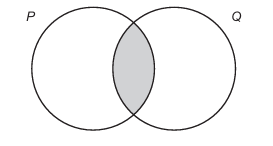
\includegraphics[width=0.4\textwidth]{images/H2-1.png} % thêm link hình tại đây
\caption*{Hình 2.1: Sơ đồ Venn cho toán tử AND}
\end{figure}

\begin{table}[H]
\centering
\renewcommand{\arraystretch}{1.3}
\begin{tabular}{|c|c|c|}
\hline
$P$ & $Q$ & $P \lor Q$ \\ \hline
Đúng & Đúng & Đúng \\ \hline
Đúng & Sai & Đúng \\ \hline
Sai & Đúng & Đúng \\ \hline
Sai & Sai & Sai \\ \hline
\end{tabular}
\caption*{Bảng 2.4: Bảng chân trị của phép tuyển (OR logic)}
\end{table}

\begin{itemize}
    \item Bảng 2.4 cho thấy rằng một phép tuyển được coi là đúng miễn là có ít nhất một mệnh đề đúng. Điều này có nghĩa là ý định trong ví dụ trước – “Món khai vị là súp hoặc salad [nhưng không phải cả hai]” – không phù hợp với ý nghĩa logic của toán tử OR (xem Hình 2.2).
\end{itemize}

\begin{figure}[H]
\centering
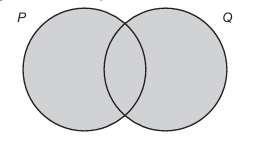
\includegraphics[width=0.4\textwidth]{images/H2-2.png} % thêm link hình tại đây
\caption*{Hình 2.2: Sơ đồ Venn cho toán tử OR}
\end{figure}

\begin{table}[H]
\centering
\renewcommand{\arraystretch}{1.3}
\begin{tabular}{|c|c|}
\hline
$P$ & $\neg P$ \\ \hline
Đúng & Sai \\ \hline
Sai & Đúng \\ \hline
\end{tabular}
\caption*{Bảng 2.5: Bảng chân trị của phép phủ định (NOT logic)}
\end{table}

\begin{itemize}
    \item Hình 2.3 biểu diễn trực quan sự khác biệt giữa một mệnh đề có và không có toán tử NOT. Nói cách khác, điều gì đúng sẽ trở thành sai, và điều gì sai sẽ trở thành đúng.
\end{itemize}

\begin{figure}[H]
\centering
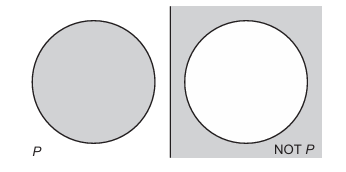
\includegraphics[width=0.4\textwidth]{images/H2-3.png} % thêm link hình tại đây
\caption*{Hình 2.3: Sơ đồ Venn cho toán tử NOT}
\end{figure}

\begin{table}[H]
\centering
\renewcommand{\arraystretch}{1.3}
\begin{tabular}{|c|c|c|}
\hline
$P$ & $Q$ & $P \rightarrow Q$ \\ \hline
Đúng & Đúng & Đúng \\ \hline
Đúng & Sai & Sai \\ \hline
Sai & Đúng & Đúng \\ \hline
Sai & Sai & Đúng \\ \hline
\end{tabular}
\caption*{Bảng 2.6: Bảng chân trị của phép kéo theo (IMPLIES logic)}
\end{table}

\begin{itemize}
    \item Hai dòng đầu của Bảng 2.6 có vẻ hợp lý. Nếu $P$ đúng kéo theo $Q$ đúng và cả hai thực sự đúng, thì phép kéo theo là hợp lệ. Tương tự, nếu $P$ đúng nhưng hệ quả của nó không đúng, thì phép kéo theo là không hợp lệ.

    \item Tuy nhiên, hai dòng cuối có vẻ kỳ lạ. Phép kéo theo vẫn hợp lệ bất kể giá trị của $P$.

        \begin{tcolorbox}
Tại sao việc $P$ kéo theo $Q$ lại hợp lệ khi $P$ sai? Trong phép " $P$ kéo theo $Q$ ", $P$ được gọi là tiền đề (antecedent) và $Q$ là hệ quả (consequent). Lời giải thích là: không thể rút ra kết luận nào về một phép kéo theo khi tiền đề (tức là $P$) sai.Hãy xem xét phát biểu: "nếu trời mưa ($P$), thì cỏ ướt ($Q$)". Việc nói rằng "trời không mưa" ($\neg P$) không mâu thuẫn với việc cỏ đang ướt. Cỏ có thể ướt vì một lý do khác, chẳng hạn như do vòi phun nước đang bật. Vì không có sự mâu thuẫn, các nhà toán học đã nhận định rằng một phép kéo theo với tiền đề sai là đúng cho đến khi có bằng chứng chứng minh ngược lại (xem Hình 2.4).
\end{tcolorbox}
\end{itemize}

\begin{itemize}
    \item Hình 2.4 là sơ đồ Venn mô tả toán tử kéo theo (IMPLIES).
\end{itemize}

\begin{figure}[H]
\centering
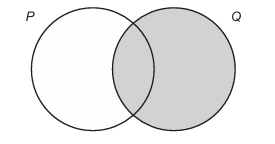
\includegraphics[width=0.4\textwidth]{images/H2-4.png} % thêm link hình tại đây
\caption*{Hình 2.4: Sơ đồ Venn cho toán tử IMPLIES}
\end{figure}

\begin{table}[H]
\centering
\renewcommand{\arraystretch}{1.3}
\begin{tabular}{|c|c|c|}
\hline
$P$ & $Q$ & $P \leftrightarrow Q$ \\ \hline
Đúng & Đúng & Đúng \\ \hline
Đúng & Sai & Sai \\ \hline
Sai & Đúng & Sai \\ \hline
Sai & Sai & Đúng \\ \hline
\end{tabular}
\caption*{Bảng 2.7: Bảng chân trị của phép tương đương (IF AND ONLY IF)}
\end{table}

\begin{itemize}
    \item Hình 2.5 mô tả toán tử IF AND ONLY IF. Chỉ khi các giá trị trùng khớp thì mệnh đề mới được coi là đúng. $P$ và $Q$ có thể trùng khớp khi giá trị của chúng giống nhau, tức là cùng đúng hoặc cùng sai.
\end{itemize}

\begin{figure}[H]
\centering
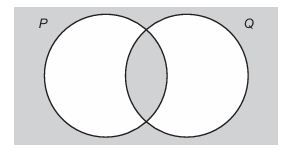
\includegraphics[width=0.4\textwidth]{images/H2-5.png} % thêm link hình tại đây
\caption*{Hình 2.5: Sơ đồ Venn cho toán tử IF AND ONLY IF}
\end{figure}



